\documentclass[specialist,
               substylefile = spbu.rtx,
               subf,href,colorlinks=true, 12pt]{disser}
\usepackage[breakable]{tcolorbox}
\usepackage[a4paper,left=3cm, right=1.5cm, top=2cm, bottom=2cm, headsep=1cm, footskip=1cm]{geometry}
\usepackage[utf8]{inputenc}
\usepackage[T2A]{fontenc}
\usepackage{graphicx}
\usepackage[english,russian]{babel}
\usepackage{amsfonts}
\usepackage{amsmath}
\usepackage{bm}
\usepackage{float}
\usepackage{amsthm}
\usepackage{parskip} % Stop auto-indenting (to mimic markdown behaviour)
\usepackage[ruled,vlined]{algorithm2e}
\newtheorem{statement}{Утверждение}
\newtheorem*{statement*}{Утверждение}
\newtheorem*{notice*}{Замечание}
\newtheorem{lemma}{Лемма}  
\newtheorem*{def*}{Определение}  

%\DeclareMathOperator{\Re}{Re}
%\DeclareMathOperator{\Im}{Im}
\DeclareMathOperator{\med}{med}
\DeclareMathOperator{\diag}{diag}
\DeclareMathOperator{\tr}{tr}
\newcommand{\tX}[1]{\mathsf{#1}}
\newcommand{\norm}[1]{\left\lVert#1\right\rVert}
\DeclareMathOperator*{\argminB}{argmin}

\geometry{verbose,tmargin=1in,bmargin=1in,lmargin=1in,rmargin=1in}

\DeclareMathOperator*{\argmin}{argmin}

\SetKwInput{KwData}{Исходные параметры}
\SetKwInput{KwResult}{Результат}
\SetKwInput{KwIn}{Входные данные}
\SetKwInput{KwOut}{Выходные данные}
\SetKwIF{If}{ElseIf}{Else}{если}{тогда}{иначе если}{иначе}{конец условия}
\SetKwFor{While}{до тех пор, пока}{выполнять}{конец цикла}
\SetKw{KwTo}{от}
\SetKw{KwRet}{возвратить}
\SetKw{Return}{возвратить}
\SetKwBlock{Begin}{начало блока}{конец блока}
\SetKwSwitch{Switch}{Case}{Other}{Проверить значение}{и выполнить}{вариант}{в противном случае}{конец варианта}{конец проверки значений}
\SetKwFor{For}{цикл}{выполнять}{конец цикла}
\SetKwFor{ForEach}{для каждого}{выполнять}{конец цикла}
\SetKwRepeat{Repeat}{повторять}{до тех пор, пока}
\SetAlgorithmName{Алгоритм}{алгоритм}{Список алгоритмов}    


\begin{document}

\institution{
    Санкт-Петербургский государственный университет \\
    Прикладная математика и информатика \\
    Вычислительная стохастика и статистические модели
}

\title{Отчет о научно-исследовательской работе}

\topic{\normalfont\scshape
  Робастные варианты метода SSA для анализа комплексных временных рядов}

\author{Сенов Михаил Андреевич}

\sa       {Н.\,Э.~Голяндина}
\sastatus {к.\,ф.-м.\,н., доцент}

\city{Санкт-Петербург}
\date{\number\year}

\maketitle


\section{Введение}
Временным рядом называется набор значений некоторой функции от времени, собранных в разные моменты времени.

Предположим, что временной ряд является суммой нескольких временных рядов, к примеру, тренда (медленно меняющейся составляющей), сезонной составляющей и шума. Для работы с таким рядом полезно выделить эти составляющие, поскольку работать с ними по отдельности может быть проще чем с исходным рядом, сделать это позволяет метод <<Гусеница>>-SSA (в дальнейшем просто SSA).

При подобном анализе возникает следующее затруднение. В данных часто возникают выделяющиеся ошибки, значительно большие, чем размер шума. Эти ошибки называются выбросами. Соответственно, возникает задача построения изначально устойчивых к выбросам модификаций SSA. 

Решению данной задачи была посвящена работа \cite{Tretyakova20}. Результаты были получены для вещественнозначных рядов. В реальности данные с многих приборов снимаются изначально в комплексном виде и, поэтому, задача анализа комплекснозначных временных рядов так же важна. Поэтому, целью данной работы является рассмотрение возможности переноса полученных ранее результатов на комплексный случай и их обобщение в случае неудачи.

\section{Алгоритм SSA}
В этом разделе рассмотрим базовый алгоритм SSA.
\subsection{Описание алгоритма}
Рассмотрим ненулевой ряд $\tX{X}_N = (x_1, \ldots, x_{N})$, где $N > 2$. Базовый алгоритм SSA выполняет разложение исходного ряда на сумму из нескольких новых рядов и осуществляется в четыре этапа. 
\subsubsection{Вложение}
Первым этапом алгоритма является построение траекторной матрицы.\\
Пусть $L$~--- некоторое целое число (\textit{длина окна}), $1 < L < N$

\textit{Траекторная матрица}~--- это матрица:
$$\mathbf{X} = \begin{pmatrix}
           x_1 & x_2 & \ldots & x_{K}\\
           x_2 & x_3 & \ldots & x_{K+1}\\
           \vdots & \vdots & & \vdots\\
           x_{L} & x_{L+1} & \ldots & x_{N}
         \end{pmatrix}, K = N - L + 1.$$
\subsubsection{Сингулярное разложение}
Вторым этапом является сингулярное разложение (SVD) траекторной матрицы ряда, оно может быть записано как:
$$\mathbf{X} = \mathbf{X}_1 + \ldots + \mathbf{X}_d$$
где $\mathbf{X}_i = \sqrt{\lambda_i}U_i V_i^T$, $\lambda_i$~--- $i$-ое собственное число по убыванию матрицы $\mathbf{X} \mathbf{X}^{\mathrm{T}}$, $U_i$~--- собственный вектор матрицы $\mathbf{X} \mathbf{X}^{\mathrm{T}}$, соответствующий $\lambda_i$, $V_i$~--- собственный вектор матрицы $\mathbf{X}^{\mathrm{T}} \mathbf{X}$, соответствующий $\lambda_i$, $d$~--- ранг матрицы $\mathbf{X}$.
\subsubsection{Группировка}
Третьим этапом является объединение в группы полученных матриц $\mathbf{X}_i$.

Матрица, соответствующая группе $I$:
$$\mathbf{X}_I = \mathbf{X}_{i_1} + \ldots + \mathbf{X}_{i_r}.$$
И результат группировки:
$$\mathbf{X} = \mathbf{X}_{I_1} + \ldots + \mathbf{X}_{I_l}.$$
\subsubsection{Диагональное усреднение}
Последним этапом является перевод каждой матрицы, соответствующей группе, в новый ряд длины $N$.

Пусть $\mathbf{Y}$ --- некоторая матрица $L \times K$ с элементами $y_{ij}$. Положим $L^* = \min(L, K)$, $K^* = \max(L, K)$, $N = L + K - 1$. Пусть $y^{*}_{ij} = y_{ij}$, если $L < K$, и $y^{*}_{ij} = y_{ji}$ иначе.

Диагональное усреднение переводит матрицу $\mathbf{Y}$ в ряд $(y_0, \ldots, y_{N - 1})$ по формуле:
$$y_k = 
 \begin{cases}
   \displaystyle{1\over{k + 1}}\sum^{k+1}_{i=1} y^{*}_{i,k - i + 2} &\text{для $0 \leq i \leq L^* - 1 $}\\
   \displaystyle{1\over{L^*}}\sum^{L^*}_{i=1} y^{*}_{i,k - i + 2} &\text{для $L^* - 1 \leq i \leq K^*$}\\
   \displaystyle{1\over{N - k}}\sum^{N - K^* + 1}_{i=k - K^* + 2} y^{*}_{i,k - i + 2} &\text{для $K^* \leq i \leq N - 1$}
 \end{cases}.$$
Таким образом, мы разложили исходный ряд в сумму $l$ новых рядов:
$$\tX{X}_N = \sum^{l}_{i = 1} \tX{X}_{N_i}.$$


\section{Робастные варианты SSA.}
В данном разделе мы рассмотрим устойчивые к выбросам (робастные) комплекснозначные модификации SSA. Особенности методов (кроме замены транспонирования $\mathrm{T}$ на эрмитово сопряжение $\mathrm{H}$) будем отмечать отдельно.

Будем рассматривать вариант метода SSA для выделения сигнала, когда группировка заключается в выборе первых $r$ компонент. Для стандартного метода SSA это эквивалентно проекции по норме Фробениуса траекторной матрицы ряда на множество матриц ранга, не превосходящего $r$.

Пусть имеется временной ряд $\tX{X_N}=(x_1, \ldots, x_{N})$.

$\mathcal{M}_{\mathcal{H}}$ --- пространство ганкелевых матриц $L\times K$,

$\mathcal{M}_{r}$ --- пространство матриц ранга, не превосходящего $r$, размера $L \times K$.

Оператор вложения $\mathcal{T}:\mathbb{R}^N(\mathbb{CС}^N) \rightarrow \mathcal{M}_{\mathcal{H}}: \mathcal{T} (\tX{X_N}) = \mathbf{X} $,

$\Pi_{r}:\mathcal{M}\rightarrow \mathcal{M}_r$ --- проектор на множество матриц ранга, не превосходящего $r$, по некоторой норме в пространстве матриц,

$\Pi_{\mathcal{H}}:\mathcal{M} \rightarrow \mathcal{M}_{\mathcal{H}}$ --- проектор на пространство ганкелевых матриц по некоторой норме в пространстве матриц.

В результате применения данных операторов получаем оценку сигнала:
\begin{equation*}
	\tilde{\tX{S}} = \mathcal{T}^{-1} \Pi_{\mathcal{H}} \Pi_{r} \mathcal{T} (\tX{X_N}).
\end{equation*}

В случае, когда проекторы $\Pi_r$ и $\Pi_{\mathcal{H}}$ берутся по норме в пространстве $\mathbb{L}_2$, оценка сигнала соответствует алгоритму SSA, для случая, когда восстановление производится по одной группе, состоящей из первых $r$ компонент.

Существует два известных подхода к построению устойчивых к выбросам модификаций SSA:

\begin{itemize}
	\item Проекторы $ \Pi_{r}$ и $\Pi_{\mathcal{H}} $ строятся по норме в пространстве $\mathbb{L}_1$,
	\item Проекторы $ \Pi_{r}$ и $\Pi_{\mathcal{H}} $ строятся по взвешенной норме в пространстве $\mathbb{L}_2$.
\end{itemize}

В работе \cite{Tretyakova20} были предложены реализации обоих подходов, приведём адаптированные на комплексный случай алгоритмы ниже. 


\subsection{Проекция по норме $\mathbb{L}_1$}

Пусть $\mathbf{Y} \in \mathbb{C}^{L\times K}$ --- траекторная матрица ряда.
Необходимо решить задачу
\begin{equation*}
	\norm{\mathbf{Y}-\mathbf{U}\mathbf{V}^{\mathrm{H}}}_1 \longrightarrow \min_{\mathbf{U},\mathbf{V}}, \, \mathbf{U} \in \mathbb{C}^{L\times r}, \mathbf{V} \in \mathbb{C}^{K\times r}.
\end{equation*}

\begin{algorithm}[H]
\SetAlgoLined
\KwIn{$\mathbf{Y} \in \mathbb{C}^{L\times K}$~--- траекторная матрица ряда, $r$~--- ранг сигнала; параметры критерия остановки: $\varepsilon = 10^{-4}$, максимальное число итераций $N_{iter} = 10$}
\KwOut{$\mathbf{\hat{Y}} = \mathbf{U}\mathbf{V}^\mathrm{H}$~--- проекция траекторной матрицы на множество матриц ранга, не превосходящего $r$}
 Инициализация $\mathbf{V}(0) \in \mathbb{C}^{L\times r}$, нормировка столбцов $\mathbf{V}(0)$\;
 $t := 0$\;
 \While{$\max\limits_{\substack{i=1,\ldots,L \\ j=1,\ldots,r}} |u_{ij} (t) - u_{ij} (t - 1)| > \varepsilon$ и $t < N_{iter}$}{
  $t := t + 1$\;
  $\mathbf{U(t)} = \argmin\limits_{\mathbf{U}\in \mathbb{C}^{L\times r}} ||\mathbf{Y} - \mathbf{U}\mathbf{V}^\mathrm{H}(t - 1)||_1$\;
  $\mathbf{V(t)} = \argmin\limits_{\mathbf{V}\in \mathbb{C}^{K\times r}} ||\mathbf{Y} - \mathbf{U}(t)\mathbf{V}^\mathrm{H}||_1$\;
  Нормировка столбцов $\mathbf{V}(t)$\;
  }
  $\mathbf{U} := \mathbf{U}(t); \mathbf{V} := \mathbf{V}(t)$\;
 \caption{Последовательный метод построения $\mathbb{L}_1$-проектора на множество матриц ранга, не превосходящего $r$}
\end{algorithm}

В приведённой реализации $\mathbf{V}(0)$ инициализируется при помощи сингулярного разложения, но, согласно~\cite{KeKanade}, инициализация может быть произведена при помощи любой матрицы требуемого размера с сохранением сходимости.  

Рассмотрим подробнее решение задачи 
\begin{equation}\label{task1}
	\mathbf{U}(t) = \argmin\limits_{\mathbf{U}\in \mathbb{C}^{K\times r}} \|\mathbf{Y}-\mathbf{U}\mathbf{V}^{\mathrm{H}}(t-1)\|_1.
\end{equation}

Целевую функцию можно представить в виде $$\|\mathbf{Y}-\mathbf{U}\mathbf{V}^{\mathrm{H}}(t-1)\|_1 = \sum\limits_{i=1}^{L} \|\mathbf{y}_i^{\mathrm{H}}-\mathbf{V}(t-1)\mathbf{u}^{\mathrm{H}}_i \|_1, $$ где $\mathbf{y}_i\in \mathbb{C}^K$ --- строки $\mathbf{Y}$, $\mathbf{v}_i\in\mathbb{C}^r$ --- строки $\mathbf{U}$.
Согласно~\cite{KeKanade}, задача~(\ref{task1}) может быть разбита на $L$ независимых подзадач
\begin{equation}\label{subtask1}
	\mathbf{u}_i(t) = \argmin\limits_{u}\|\mathbf{y}_i^{\mathrm{H}}-\mathbf{V}(t-1)\mathbf{u}^{\mathrm{H}} \|_1.
\end{equation}
 Подзадача~(\ref{subtask1}) в свою очередь может быть разбита на $r$ подзадач
\begin{equation}\label{subtask1}
	\mathbf{u}_{ic}(t) = \argmin\limits_{u_c}\|\mathbf{y}_{i}^{\mathrm{H}}-\mathbf{v}_c(t-1)\mathbf{u_c}^{\mathrm{H}} \|_1.
\end{equation}
Решение каждой из которых является взвешенной медианой вектора $\frac{\mathbf{y}_i}{\mathbf{v}_c(t-1)}$ с вектором весов $|\mathbf{v}_c(t-1)|$.

\subsection{Проекция по взвешенной норме $\mathbb{L}_2$ с итеративным обновлением весов}

Пусть $\mathbf{Y} \in \mathbb{C}^{L\times K}$ --- траекторная матрица ряда.
Необходимо решить задачу
\begin{equation*}
		\norm{\mathbf{W}^{1/2}\odot(\mathbf{Y}-\mathbf{U}\mathbf{V}^{\mathrm{H}})}^2_F \longrightarrow \min_{\mathbf{U},\mathbf{V}}, \, \mathbf{U} \in \mathbb{C}^{L\times r}, \mathbf{V} \in \mathbb{C}^{K\times r}. 
\end{equation*}

Для начала рассмотрим алгоритм с фиксированной матрицей весов.

\begin{algorithm}[H]\label{alg}
	\SetAlgoLined
	\KwIn{$\mathbf{Y} \in \mathbb{C}^{L\times K}$ --- траекторная матрица ряда, $r$ --- ранг сигнала,  $\mathbf{W} \in \mathbb{R}^{L\times K}$ --- матрица весов; ~~~~~~~~~~~~~~~~~~~~~~~~~~~~~~ параметры критерия остановки:  $\varepsilon = 10^{-4}$, ~~~~~~~~~~~~~ максимальное число итераций $N_\alpha = 5$}
	\KwOut{$\widehat{\mathbf{Y}} = \mathbf{U}\mathbf{V}^{\mathrm{H}}$ --- решение задачи взвешенной аппроксимации при фиксированной матрице весов $\mathbf{W}$}
	
	1. $t:=0$\;
	2. \While{ $\norm{\mathbf{W}^{1/2}\odot(\mathbf{Y}-\mathbf{U}\mathbf{V}^{\mathrm{H})}}^2_F > \varepsilon\text{~и~} \text{t}< N_\alpha$}{
		a. Вычисление матрицы $\mathbf{U}\in \mathbb{C}^{L\times r}$ с помощью решения задачи
		\begin{equation}\label{taskA}
			(y_i^\mathrm{H}-\mathbf{V}u_i^\mathrm{H})^\mathrm{H} \mathbf{W}_i (y_i^\mathrm{H}-\mathbf{V}u_i^\mathrm{H}) \to \min_{u_i},~~ i=1,\ldots L,
		\end{equation} 
		где $\mathbf{W}_i=\diag(w_i)\in \mathbb{R}^{K\times K}$ --- матрица, составленная из $i$-ой строки $\mathbf{W}$\;
		b. Вычисление матрицы $\mathbf{V}\in \mathbb{C}^{K\times r}$ с помощью решения задачи
		\begin{equation}\label{taskB}
			(y_j-\mathbf{U}v_j^\mathrm{H})^\mathrm{H} \mathbf{W}^j (y_j-\mathbf{U}v_j^\mathrm{H}) \to \min_{v_j},,~~ j=1,\ldots K,
		\end{equation} 
		где $\mathbf{W}^j=\diag(W_j)\in \mathbb{R}^{L\times L}$ --- матрица, составленная из $j$-го столбца $\mathbf{W}$\;
		c. $t:=t+1$.	
	}
	\caption{Алгоритм решения задачи взвешенной аппроксимации для фиксированной матрицы весов $\mathbf{W}$}
\end{algorithm}

Задачи~(\ref{taskA}), (\ref{taskB}) решаются при помощий QR-разложения матриц $\mathbf{V}^\mathrm{H}\mathbf{W}_i\mathbf{V}$ и $\mathbf{U}^\mathrm{H}\mathbf{W}^j\mathbf{U}$ соответственно, алгоритм решения представлен в \cite{IRLS}.

У авторов этого алгоритма в \cite{Chen} допущена ошибка в его описании. Дело в том, что в задаче \ref{taskA} решение линейного уравнения ищется по эрмитово-сопряжённой системе, а не изначальной, а в задаче \ref{taskB} находится сразу $\mathbf{V}^\mathrm{H}$, а не $\mathbf{V}$. Эта ошибка была несущественной в случае вещественной реализации в \cite{Tretyakova20}, так как вещественный аналог эрмитового сопряжения~--- транспонирование, не меняет элементы, но оказалась существенной в комплексном случае. 

Теперь рассмотрим алгоритм с итеративным обновлением весов.

\begin{algorithm}[H]
\SetAlgoLined
\KwIn{$\mathbf{Y} \in \mathbb{C}^{L\times K}$~--- траекторная матрица ряда, $r$~--- ранг сигнала; параметр весовой функции $\alpha = 4.685$; параметры критерия остановки: $\varepsilon = 10^{-4}$, максимальное число итераций $N_{iter} = 10$}
\KwOut{$\mathbf{\hat{Y}} = \mathbf{U}\mathbf{V}^\mathrm{H}$~--- проекция траекторной матрицы на множество матриц ранга, не превосходящего $r$}
 Инициализация $\mathbf{U} \in \mathbb{C}^{L\times r}$ и $\mathbf{V}(0) \in \mathbb{C}^{K\times r}$ (например, с помощью сингулярного разложения матрицы $\mathbf{Y}$)\;
 $t := 0$\;
 \While{$||\mathbf{W}^\frac{1}{2} \odot (\mathbf{Y} - \mathbf{U}\mathbf{V}^\mathrm{H})||_{F}^{2} > \varepsilon$ и {$t < N_{iter}$}}{
  Вычисление матрицы остатков $\mathbf{R} = \{r_{ij}\}_{i,j=1}^{n,p} = \mathbf{Y} - \mathbf{U}\mathbf{V}^\mathrm{H}$\;
  Обновление матрицы $\mathbf{\Sigma} = \{\sigma_{ij}\}^{L,K}_{i,j=1}$\;
  Вычисление матрицы весов $\mathbf{W} = \{w_{ij}\}^{L,K}_{i,j=1} = \{w(\frac{r_{ij}}{\sigma_{ij}})\}^{L,K}_{i,j=1}$, используя
  $$w(x) = 
 \begin{cases}
   (1 - (\frac{|x|}{\alpha})^2)^2 &|x| \leq \alpha\\
   0 &|x| > \alpha\\
 \end{cases};$$
 Решение задачи взвешенной аппроксимации (обновление матриц $\textbf{U}$, $\textbf{V}$)
 $$||\mathbf{W}^\frac{1}{2} \odot (\mathbf{Y} - \mathbf{U}\mathbf{V}^\mathrm{H})||_{F}^{2} \longrightarrow \min_{\textbf{U}, \textbf{V}},$$
 при помощи алгоритма \ref{alg}\;
  }
 \caption{Метод с итеративным обновлением весов для нахождения про-
екции на множество матриц ранга, не превосходящего $r$}
\end{algorithm}

Данный алгоритм был предложен в \cite{Chen}, авторы предложили взять $\alpha = 4.685$, $N_{\alpha} = 5$ и $N_{iter} = 10$, ссылаясь на численные эксперементы.

Параметр сигма предлагается взять равным $\sigma_{ij} = \sigma = 1.4826 \med {|\tX{R}-\med {|\tX{R}|}|}$, где $\tX{R}$~--- это вектор, составленный из всех элементов матрицы остатков $\mathbf{R} = \{r_{ij}\}_{i,j=1}^{L,K}$, то есть
\begin{equation*}
	\tX{R}~=~(r_{11},\ldots,r_{1K}; r_{21},\ldots r_{2K};\ldots;r_{L1},\ldots,r_{LK}).
\end{equation*} 
Данная оценка предлагается авторами ввиду её робастности.

\subsection{Модификация метода с итеративным обновлением весов}

У представленного выше алгоритма есть одна важная проблема, а именно, выбор параметра $\sigma_{ij}$ не зависящим от $i$ и $j$. В случае не стационарных рядов выявление выбросов может происходить неверно. Например, если шум растёт к концу ряда, то выбросы в начале ряда могут получить больший вес, чем не выбросы в конце ряда. В \cite{Tretyakova20} была приведена модификация алгоритма, призванная решить эту проблему. Здесь же мы рассмотрим её комплексную адаптацию.

Ключевая задача параметра $\sigma_{ij}$~--- приписывание определённого веса определённому элементу ряда, чем элемент больше похож на выброс, тем больше сигма и наоборот. Ввиду такой интерпретации логично рассматривать сигмы как ряд, идущий дополнением к данному $\bm{\sigma} = (\sigma_1,\ldots,\sigma_N)$, а после, ганкелизацией привести этот ряд к матричному виду $\mathbf{\Sigma}=\{\sigma_{ij}\}_{i,j=1}^{L,K}$. Сам же ряд $\bm{\sigma}$ автор \cite{Tretyakova20} предлагает взять равным тренду (математическому ожиданию) ряда из модулей остатков. Это предложение справедливо и для комплексного случая, так как в комплексном случае выброс характеризуется величиной модуля.

Теперь рассмотрим сам алгоритм.

\small{
	\begin{algorithm}[H]
		\SetAlgoLined
		\KwIn{$\mathbf{Y} \in \mathbb{C}^{L\times K}$ --- траекторная матрица ряда, $r$ --- ранг сигнала;
			параметр весовой функции $\alpha = 4.685$; параметры критерия остановки: $\varepsilon = 10^{-4}$, максимальное число итераций $N_{iter} = 10$}
		\KwOut{$\widehat{\mathbf{Y}} = \mathbf{U}\mathbf{V}^{\mathrm{T}}$ --- проекция траекторной матрицы на множество матриц ранга, не превосходящего $r$}
		
		1. Инициализация $\mathbf{U}\in \mathbb{C}^{L\times r}$ и $\mathbf{V}\in \mathbb{C}^{K\times r}$ (например, с помощью сингулярного разложения матрицы $\mathbf{Y}$)\;
		2. $t:=0$\;
		3. \Repeat{ $\norm{\mathbf{W}^{1/2}\odot(\mathbf{Y}-\mathbf{U}\mathbf{V}^{\mathrm{H}})}^2_F > \varepsilon \text{~и~} t < N_{IRLS}$}{
			a. Вычисление матрицы остатков $\mathbf{R}=\{r_{ij}\}_{i,j=1}^{n,p} = \mathbf{Y}-\mathbf{U}\mathbf{V}^\mathrm{H}$\;
			b. Ганкелизация матрицы $\mathbf{R}$ и получение ряда длины $N$ из остатков: $\tX{R} = \mathcal{T}^{-1} \Pi_{\mathcal{H}} (\mathbf{R}) = (r_1,\ldots,r_N)$\;
			c. Пусть $\tX{R}_+=(|r_1|, \ldots, |r_N|)$~--- ряд из модулей остатков.  Вычисление $\bm{\sigma} = (\sigma_1,\ldots,\sigma_{N})$ как оценки мат. ожидания $\mathbb{E}(\tX{R}_+)$ некоторым методом;
			
			d. Получение матрицы $\mathbf{\Sigma} = \{\sigma_{ij}\}_{i,j=1}^{L,K} = \mathcal{T} (\sigma)$\;
			e. Вычисление матрицы весов $\mathbf{W} = \{w_{ij}\}^{L,K}_{i,j=1} = \{w(\frac{r_{ij}}{\sigma_{ij}})\}^{L,K}_{i,j=1}$, используя %$w(x)=\frac{\partial \rho(x)}{\partial |x|} \frac{1}{|x|}$:
			\begin{equation*}
				w(x) = 
				\begin{cases}
					(1-(\frac{|x|}{\alpha})^2)^2, &|x|\le\alpha\\
					0, &|x|>\alpha
				\end{cases}\; %~~~ \text{где}~ x=r^*.
				\; \end{equation*} 
			f. Решение задачи взвешенной аппроксимации (обновление матриц $\mathbf{U}$ и $\mathbf{V}$)
			\begin{equation*}
				\norm{\mathbf{W}^{1/2}\odot(\mathbf{Y}-\mathbf{U}\mathbf{V}^{\mathrm{H}})}^2_F \longrightarrow \min_{\mathbf{U},\mathbf{V}}\;
			\end{equation*}	
			g. $t:=t+1$.
		}
		\caption{Модификация метода с итеративным обновлением весов для нахождения проекции на множество матриц ранга, не превосходящего $r$}
	\end{algorithm}
}

%\normalsize{Приведём пример, показывающий, что алгоритм действительно присваивает правильные веса в случае %нестационарного шума.}

\normalsize{Преимуществом данного алгоритма, является то, что пользователь сам может выбрать, каким методом он хочет вычислять матожидание ряда. В приведённой реализации представлены три метода: локальная регрессия loess, скользящая медиана и взвешенная локальная регрессия lowess.}

%\subsection{Трудоёмкость методов}
%
%
%\subsubsection{Проекция по норме $\mathbb{L}_2$}
%Трудоёмкость обычной, не робастной проекции по норме $\mathbb{L}_2$ была рассмотрена в \cite{Chen} и составляет
%\begin{equation*}
%	\mathrm{T}_{\mathrm{cssa}} = O(LK^2).
%\end{equation*}
%
%\begin{notice*}
% Complex SSA из пакета rssa, который мы будем использовать, на самом деле работает быстрее, ввиду того, что SVD в нём %вычисляется не до конца.
%\end{notice*}
%
%\subsubsection{Проекция по норме $\mathbb{L}_1$}
%Трудоёмкость вычисления взвешенной медианы для вектора длины $n$ составляет $O(n)$, при решении задачи \ref{task1} вектор %имеет длину $K$, а медиана считается $Lr$ раз. Задача \ref{task1} решается не более чем $N_{iter}$ раз. Итого, получаем %оценку трудоёмкости
%\begin{equation*}
%	\mathrm{T}_{\mathrm{l1}} = O(L K r N_{iter}).
%\end{equation*}
%
%\subsubsection{Взвешенная проекция по норме $\mathbb{L}_2$}
%Трудоёмкость метода была рассмотрена в \cite{Chen} и составляет
%\begin{equation*}
%	\mathrm{T}_{\mathrm{weighted\,l2}} = O(L K r^2 N_{\alpha} N_{iter}).
%\end{equation*}
%
%\subsubsection{Сравнение теоретической трудоёмкости методов}
%Из представленных результатов видно, что оба робастных метода быстрее навиной реализации неробастного метода при %достаточно большой траекторной матрице с достаточно небольшим рангом. $\mathbb{L}_1$ же показывает себя быстрее %взвешенного $L_2$ при большом ранге и/или сильно отличающимся числе итераций. Однако, вышесказанное верно только при %предположении, что число итераций не зависит от размера матрицы, что, вообще говоря, не доказано. 

%\subsubsection{Сравнение времени выполнения реализаций}
%
%Фактическое время выполнения реализаций методов для различных длин ряда рассмотрено в таблице %\ref{tab}
%
%\begin{table}
%	\caption{Сравнение времени работы алгоритмов для различных длин ряда.}
%	\label{tab}
%	\centering
%	\begin{tabular}{|c|c|c|c|c|c|}
%		\hline
%		Method 	& $N = 240$ & $N = 360$ & $N = 480$ & $N = 600$ & $N = 720$  \\ 
%		\hline
%		CSSA & 0.01s  & 0.06  & 0.13 & 0.25 & 0.34 \\
%		\hline
%		L1 & 0.86s  & 1.33  & 1.78 & 2.15 & 2.78 \\
%		\hline
%		L2-W & 1.7sec  & 5.02  & 9.66 & 16.11 & 25.44 \\
%		\hline
%	\end{tabular}
%\end{table}

\section{Примеры работы алгоритмов}
В данном разделе мы приведём несколько примеров комплексных временных рядов и сравним результаты работы методов.

Сравнение будет проводиться по величине среднеквадратичной ошибки, согласованной с $\mathbb{L}_2$, которая вычисляется по формуле
\begin{equation}\label{MSE}
	\text{MSE} = \mathbb{E} \left(\frac{1}{N} \sum \limits_{i=1}^{N}(s_i - \hat s_i )^2 \right),
\end{equation}
где $\tX{S}=(s_1,\ldots,s_N)^\mathrm{T}$ --- сигнал, $\hat{\tX{S}}=(\hat{s}_1,\ldots,\hat{s}_N)^\mathrm{T}$ --- его оценка.
Будем вычислять
\begin{equation*}
	\text{RMSE} = \sqrt{\textrm{MSE}}.
\end{equation*}

Так же будем проверять значимость сравнения, для этого будем использовать гипотезу, что MSE для некоторых методов равны между собой.

$\mathrm{H}_0: \mathbb{E}(\xi_1-\xi_2)=0$.
Имеем две выборки $X=(x_1,\ldots,x_M)$ и $Y=(y_1,\ldots,y_M)$ объема $M$. Обозначим $\bar{X}$ и $\bar{Y}$ --- их выборочные средние, $s_x^2$ и $s_y^2$ --- выборочные дисперсии, $\hat\rho$ --- коэффициент корреляции. 
Статистика критерия 
\begin{equation*}
	t = \frac{\sqrt{M}(\bar{X}-\bar{Y})}{\sqrt{s_x^2+s_y^2-2s_xs_y\hat\rho}}
\end{equation*}
имеет асимптотически нормальное распределение.

Шум в примерах будет иметь стандартное комплексное нормальное распределение. Определим, что это значит.
\begin{def*}
	Комплексная случайная величина $Z$ имеет стандартное комплексное нормальное распределение, если
	\begin{enumerate}
		\item $\Re(Z)$ и $\Im(Z)$ независимы,
		\item $\Re(Z), \, \Im(Z) \sim N(0, 1/2)$.
	\end{enumerate}
	И обозначается $Z \sim CN(0, 1)$. 
\end{def*}


\subsection{Синтетический пример №1}

Рассмотрим ряд с постоянной амплитудой и шумом постоянной дисперсии.
Длину ряда возьмём $N = 240$
$$x_n = e^{2n\pi/30i} + \varepsilon_n, ~ \varepsilon_n \sim CN(0,1).$$
 
Рассмотрим результаты работы методов для такого ряда (\ref{tab1}). В таблице \ref{tab: pval1} представлены p-value для сравнения методов с лучшим. Ранг ряда равен 1.

\begin{table}[H]
	\begin{center}
		\caption{Оценки RMSE различных методов для $M = 30$ реализаций ряда без выбросов.}
		\label{tab1}
		\begin{tabular}{|c|c|c|c|c|c|c|}
			\hline
			Method 	& CSSA & L1 & weighted L2 & loess L2 & median L2 & lowess L2 \\ 
			\hline
			RMSE & $\mathbf{0.1016}$  & 0.125  & 0.1017 & 0.103 & 0.105 & 0.104\\
			\hline
		\end{tabular}
	\end{center}
\end{table}

\begin{table}[H]
	\caption{p-value для сравнения различных методов с наилучшим без выбросов.}
	\label{tab: pval1}
	\begin{center}
		\begin{tabular}{|c|c|c|c|c|c|}
			\hline
			Method & L1 & weighted L2 & loess L2 & median L2 & lowess L2  \\ 
			\hline
			CSSA & 1.5e-06   & \textbf{0.91} & \textbf{0.69}  & \textbf{0.24} & \textbf{0.43}  \\
			\hline
		\end{tabular} \\
	\end{center}
\end{table}

В случае отсутствия выбросов лучший результат показывают метод Complex SSA, но сравнение значимо только с методом проекции на $\mathbb{L}_1$.

Теперь добавим к ряду $5\%$ выбросов с величиной выброса $5x_i$. Графики ряда представлены на Рис. \ref{ser_Re_1}, \ref{ser_Im_1}.

\begin{figure}[H]
	\begin{center}
		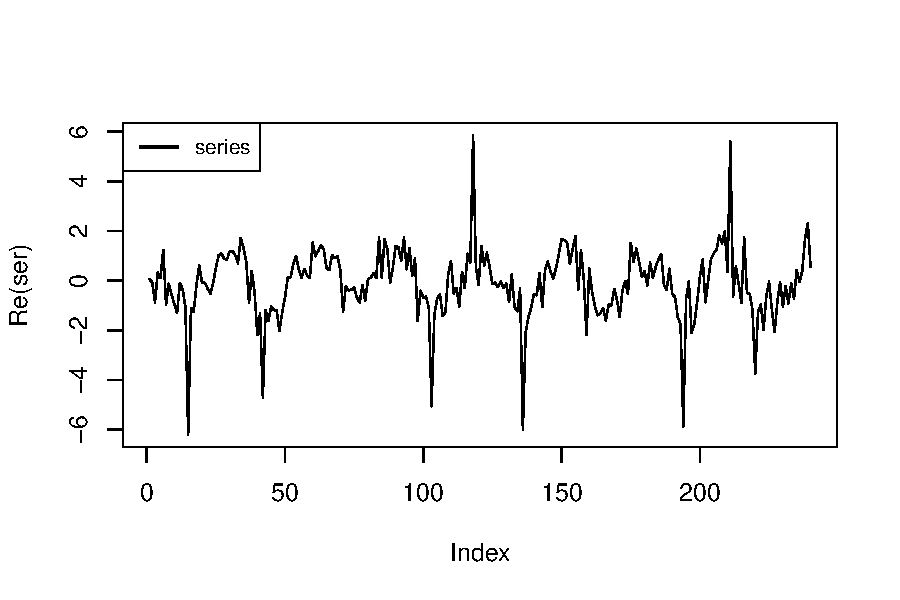
\includegraphics[width=0.5\linewidth]{ser_1_Re.pdf}
	\end{center}
	\caption{График вещественной части ряда.}
	\label{ser_Re_1}
\end{figure}

\begin{figure}[H]
	\begin{center}
		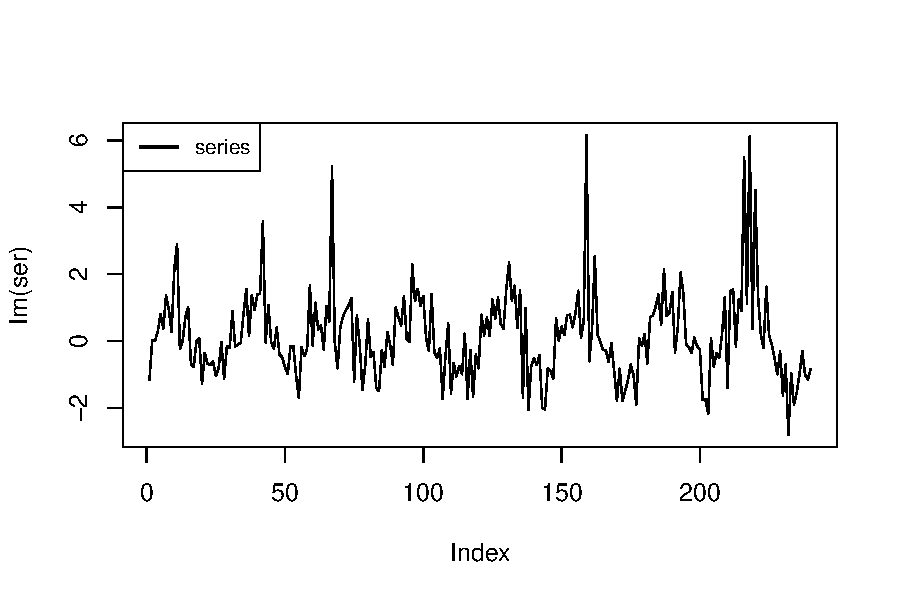
\includegraphics[width=0.5\linewidth]{ser_1_Im.pdf}
	\end{center}
	\caption{График мнимой части ряда.}
	\label{ser_Im_1}
\end{figure}

Графики результатов анализа представлены в Рис. \ref{analys_Re_1}, \ref{analys_Im_1}. В таблице \ref{tab2} представлены сравнения ошибок для различных методов.  В таблице \ref{tab: pval2} представлены p-value для сравнения методов с лучшим. Длина окна взята $L = 120$.

\begin{figure}[H]
	\begin{center}
		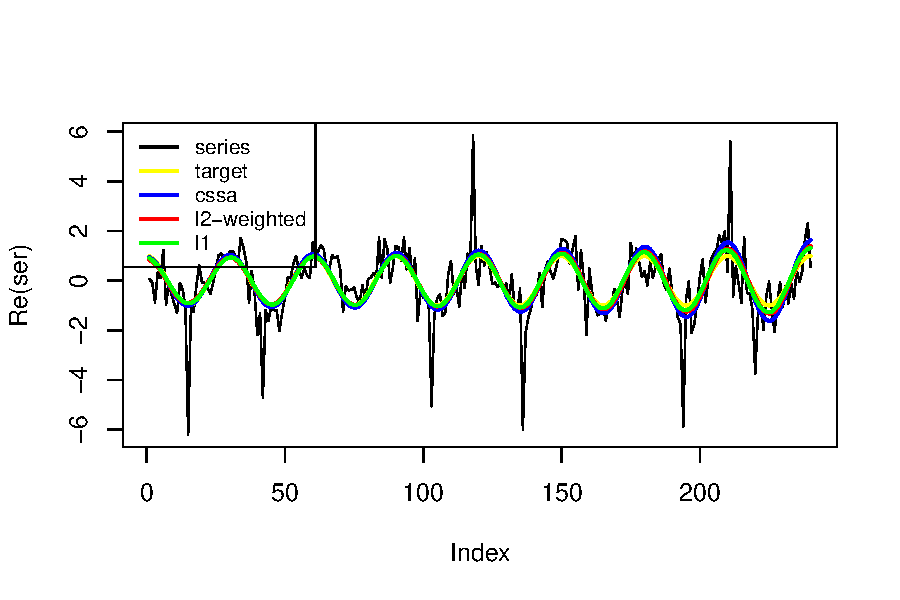
\includegraphics[width=0.5\linewidth]{analys_1_Re.pdf}
	\end{center}
	\caption{Вещественная часть выделения тренда несколькими способами.}
	\label{analys_Re_1}
\end{figure}

\begin{figure}[H]
	\begin{center}
		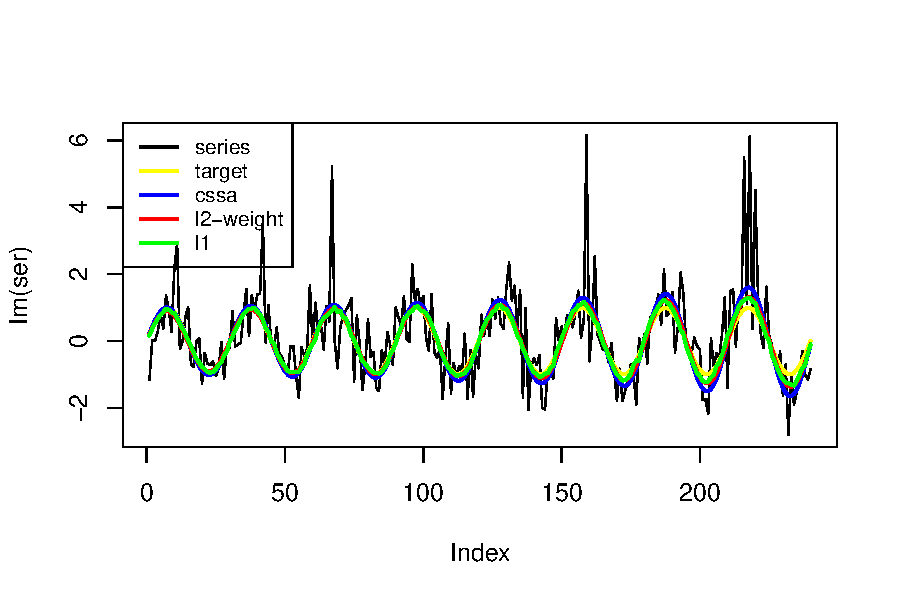
\includegraphics[width=0.5\linewidth]{analys_1_Im.pdf}
	\end{center}
	\caption{Мнимая часть выделения тренда несколькими способами.}
	\label{analys_Im_1}
\end{figure}

\begin{table}[H]
	\begin{center}
		\caption{Оценки RMSE различных методов для $M = 30$ реализаций ряда с выбросами.}
		\label{tab2}
		\begin{tabular}{|c|c|c|c|c|c|c|}
			\hline
			Method 	& CSSA & L1 & weighted L2 & loess L2 & median L2 & lowess L2 \\ 
			\hline
			RMSE & 0.285  & 0.147  & 0.158 & $\mathbf{0.112}$ & 0.114 & 0.114\\
			\hline
		\end{tabular}
	\end{center}
\end{table}

\begin{table}[H]
	\caption{p-value для сравнения различных методов с наилучшим с выбросами.}
	\label{tab: pval2}
	\begin{center}
		\begin{tabular}{|c|c|c|c|c|c|}
			\hline
			Method & CSSA	& L1 & weighted L2 & median L2 & lowess L2  \\ 
			\hline
			loess L2 & 0  & 7.7e-13 &   4.1e-10  &  \textbf{0.134} & \textbf{0.262}  \\
			\hline
		\end{tabular} \\
	\end{center}
\end{table}

В случае наличия выбросов метод loess проекции на $\mathbb{L}_2$ показал наилучший результат, за исключением того, что сравнения с другими вариациями модифицированной взвешенной проекции незначимы.


\subsection{Синтетический пример №2}

Рассмотрим ряд с растущей амплитудой и шумом непостоянной дисперсии.
Длину ряда возьмём $N = 240$
$$x_n = e^{4n/N} e^{2n\pi/30i} + \frac{1}{2}e^{4n/N} \varepsilon_n, ~ \varepsilon_n \sim CN(0,1).$$ 
Рассмотрим результаты работы методов для такого ряда (\ref{tab3}).  В таблице \ref{tab: pval3} представлены p-value для сравнения методов с лучшим. Ранг ряда равен 1.

\begin{table}[H]
	\begin{center}
		\caption{Оценки RMSE различных методов для $M = 30$ реализаций ряда без выбросов.}
		\label{tab3}
		\begin{tabular}{|c|c|c|c|c|c|c|}
			\hline
			Method 	& CSSA & L1 & weighted L2 & loess L2 & median L2 & lowess L2 \\ 
			\hline
			RMSE & $\mathbf{1.28}$  & 1.52  & 1.90 & 1.36 & 1.43 & 1.37\\
			\hline
		\end{tabular}
	\end{center}
\end{table}

\begin{table}[H]
	\caption{p-value для сравнения различных методов с наилучшим без выбросов.}
	\label{tab: pval3}
	\begin{center}
		\begin{tabular}{|c|c|c|c|c|c|}
			\hline
			Method & L1 & weighted L2 & loess L2 & median L2 & lowess L2  \\ 
			\hline
			CSSA & 0.005   & 0.0001 & 0.001  & 7.6e-5 & 0.0007  \\
			\hline
		\end{tabular} \\
	\end{center}
\end{table}

В случае отсутствия выбросов лучший результат показывает Complex SSA. Здесь же видно, что модифицированный метод взвешенной проекции справляется с не стационарным рядом куда лучше чем классический, к примеру, сравнивая классический и loess, сравнение является значимым с p-value $ = 0.0005$. 

Теперь добавим к ряду $5\%$ выбросов с величиной выброса $5x_i$. Графики ряда представлены на Рис. \ref{ser_Re_2}, \ref{ser_Im_2}.

\begin{figure}[H]
	\begin{center}
		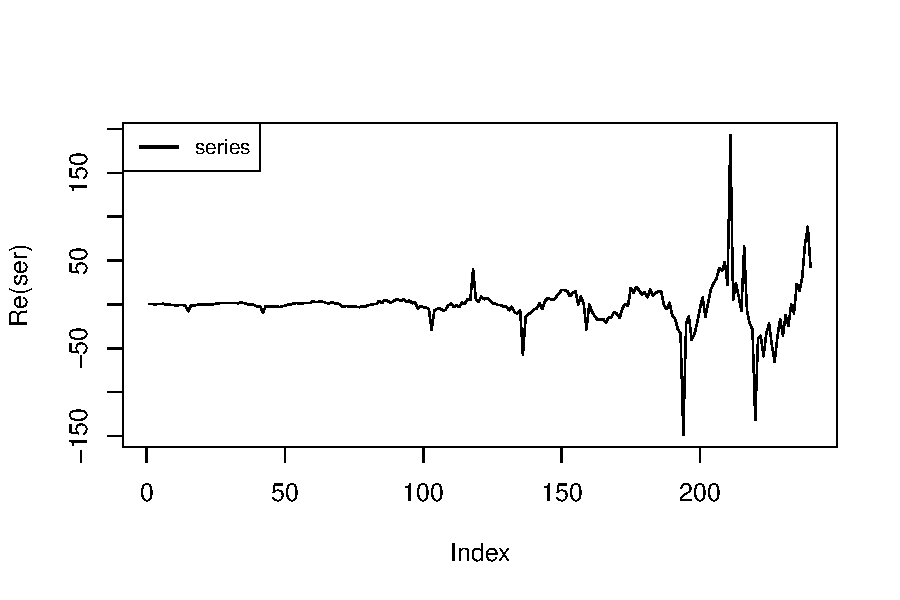
\includegraphics[width=0.5\linewidth]{ser_2_Re.pdf}
		\caption{График вещественной части ряда.}
		\label{ser_Re_2}
	\end{center}
\end{figure}

\begin{figure}[H]
	\begin{center}
		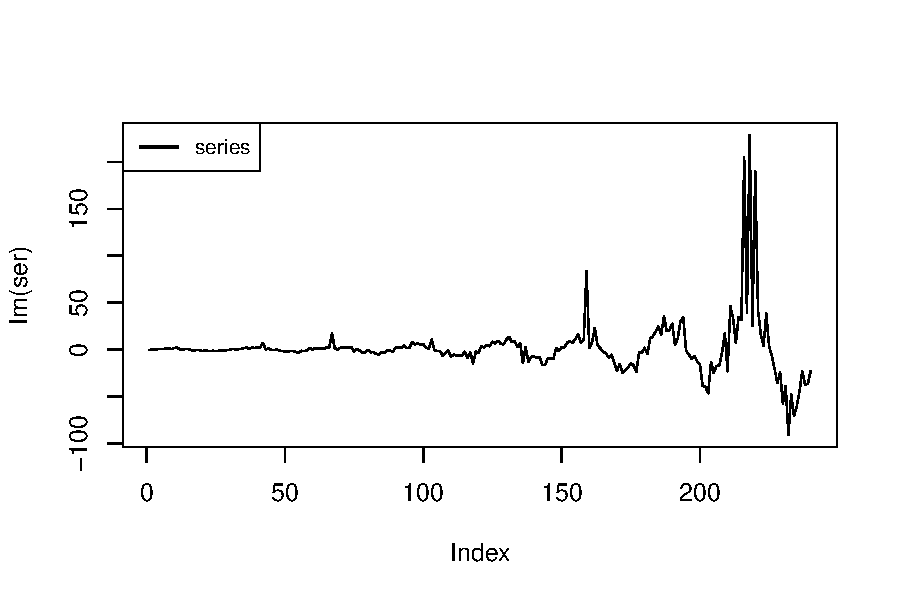
\includegraphics[width=0.5\linewidth]{ser_2_Im.pdf}
		\caption{График мнимой части ряда.}
		\label{ser_Im_2}
	\end{center}
\end{figure}

Графики результатов анализа представлены на Рис. \ref{analys_Re_2}, \ref{analys_Im_2}. В таблице \ref{tab4} представлены сравнения ошибок для различных методов. В таблице \ref{tab: pval4} представлены p-value для сравнения методов с лучшим. Длина окна взята $L = 120$.

\begin{figure}[H]
	\begin{center}
		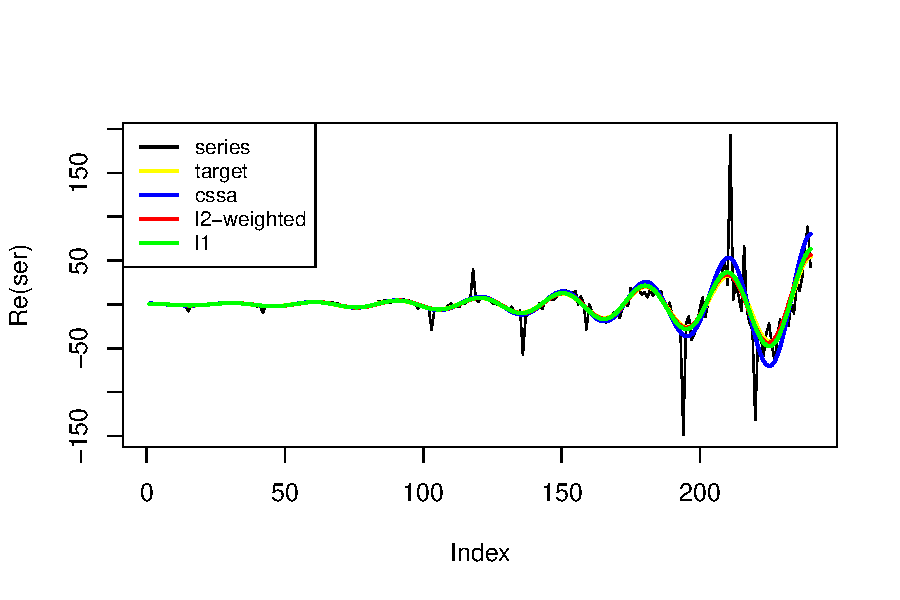
\includegraphics[width=0.5\linewidth]{analys_2_Re.pdf}
		\caption{Вещественная часть выделения тренда несколькими способами.}
		\label{analys_Re_2}
	\end{center}
\end{figure}

\begin{figure}[H]
	\begin{center}
		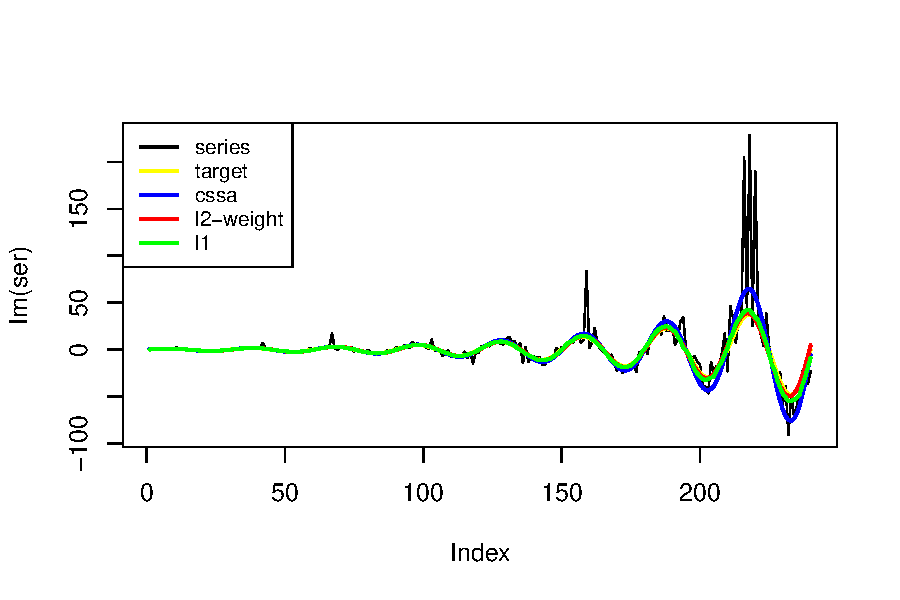
\includegraphics[width=0.5\linewidth]{analys_2_Im.pdf}
		\caption{Мнимая часть выделения тренда несколькими способами.}
		\label{analys_Im_2}
	\end{center}
\end{figure}

\begin{table}[H]
	\begin{center}
		\caption{Оценки RMSE различных методов для $M = 30$ реализаций ряда с выбросами.}
		\label{tab4}
		\begin{tabular}{|c|c|c|c|c|c|c|}
			\hline
			Method 	& CSSA & L1 & weighted L2 & loess L2 & median L2 & lowess L2 \\ 
			\hline
			RMSE & 6.14  & 1.78  & 1.66 & $\mathbf{1.48}$ & 1.50 & 1.49\\
			\hline
		\end{tabular}
	\end{center}
\end{table}

\begin{table}[H]
	\caption{p-value для сравнения различных методов с наилучшим с выбросами.}
	\label{tab: pval4}
	\begin{center}
		\begin{tabular}{|c|c|c|c|c|c|}
			\hline
			Method & CSSA	& L1 & weighted L2 & median L2 & lowess L2  \\ 
			\hline
			loess L2 & 3.5e-16   & 0.005 &   \textbf{0.13}  &  \textbf{0.387} & \textbf{0.28}  \\
			\hline
		\end{tabular} \\
	\end{center}
\end{table}

В случае присутствия выбросов метод loess проекции на $\mathbb{L}_2$ показывает себя наилучшим образом на данном примере, однако сравнения с взвешенным $\mathbb{L}_2$, median $\mathbb{L}_2$ и lowess $\mathbb{L}_2$ не являются значимыми.

\subsection{Синтетический пример №3}

При построении комплексных робастных методов возникает вопрос: Что считать выбросом? В данной работе выброс считается как элемент с аномально большим модулем. В связи с этим возникает другой вопрос: Не могут ли возникнуть проблемы в случае несимметричности распределения модуля выброса по вещественной и мнимой части? То есть не может ли получиться такой ситуации, что алгоритм посчитает выбросом точку, имеющую очень большое отклонение по вещественной оси, но на мнимой оси эта точка выбросом не является, что приведёт к ухудшению выделения тренда по мнимой оси.
 
Для рассмотрения примера на тему возьмём прошлый ряд, но выбросы сосредоточим только на вещественной оси, их вещественную часть оставив прежней. Так же в данном примере будет осмыслено посчитать помимо совместных ошибок ещё и отдельно ошибки вещественной и мнимой частей.

Графики выделения тренда представлены на Рис. \ref{analys_Re_3}, \ref{analys_Im_3}. Результаты RMSE для примера представлены в таблице \ref{tab5}. Так же посчитаем RMSE отдельно для вещественной и мнимой части для прошлого примера, для которого выбросы по модулю сделаем равными текущим, результат в таблице \ref{tab6}.
%Значения p-value представлены в таблице \ref{tab: pval5}. 

\begin{figure}[H]
	\begin{center}
		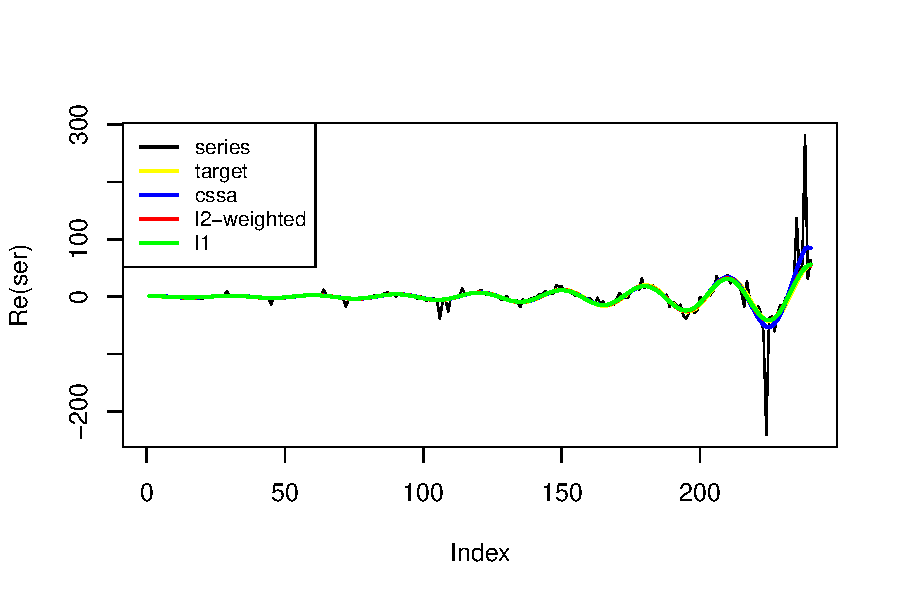
\includegraphics[width=0.5\linewidth]{analys_3_Re.pdf}
		\caption{Вещественная часть выделения тренда несколькими способами.}
		\label{analys_Re_3}
	\end{center}
\end{figure}

\begin{figure}[H]
	\begin{center}
		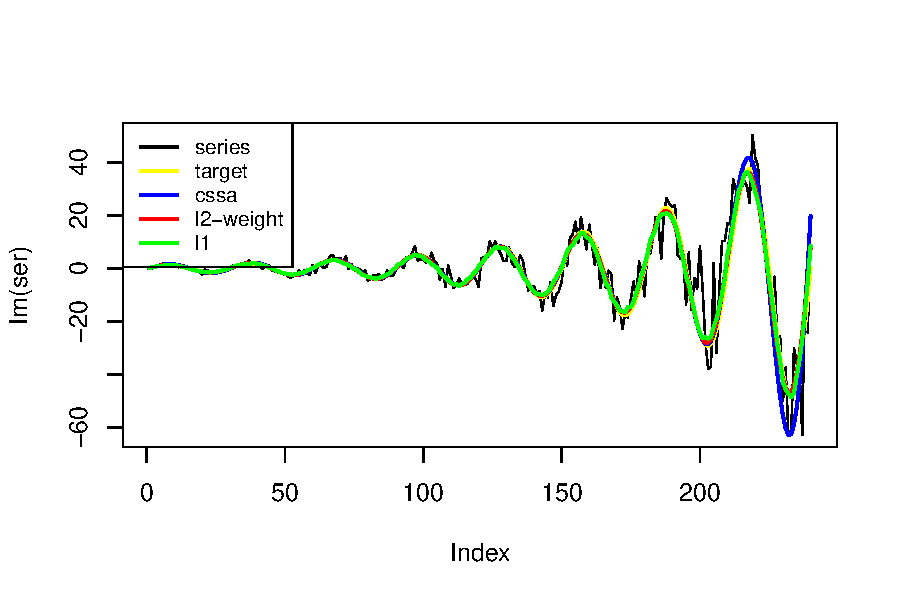
\includegraphics[width=0.5\linewidth]{analys_3_Im.pdf}
		\caption{Мнимая часть выделения тренда несколькими способами.}
		\label{analys_Im_3}
	\end{center}
\end{figure}

\begin{table}[H]
	\begin{center}
		\caption{Оценки RMSE различных методов для $M = 30$ реализаций ряда с вещественными выбросами.}
		\label{tab5}
		\begin{tabular}{|c|c|c|c|c|c|c|}
			\hline
			Method 	& CSSA & L1 & weighted L2 & loess L2 & median L2 & lowess L2 \\ 
			\hline
			RMSE (совм.) & 3.53  & 1.55  & 1.72 & $\mathbf{1.45}$ & 1.48 & 1.46\\
			\hline
			RMSE (Re) & 2.63  & 1.06  & 1.23 & $\mathbf{1.05}$ & 1.07 & 1.06\\
			\hline
			RMSE (Im) & 2.33  & 1.14  & 1.2 & $\mathbf{0.98}$ & 1.02 & 1\\
			\hline
		\end{tabular}
	\end{center}
\end{table}

\begin{table}[H]
	\begin{center}
		\caption{Оценки RMSE различных методов для $M = 30$ реализаций прошлого примера.}
		\label{tab6}
		\begin{tabular}{|c|c|c|c|c|c|c|}
			\hline
			Method 	& CSSA & L1 & weighted L2 & loess L2 & median L2 & lowess L2 \\ 
			\hline
			RMSE (совм.) & 3.53  & 1.29  & 1.34 & $\mathbf{0.97}$ & 1 & 0.98\\
			\hline
			RMSE (Re) & 2.5  & 0.85  & 0.95 & $\mathbf{0.7}$ & 0.71 & $\mathbf{0.7}$\\
			\hline
			RMSE (Im) & 2.5  & 0.97  & 0.95 & $\mathbf{0.69}$ & 0.71 & $\mathbf{0.7}$\\
			\hline
		\end{tabular}
	\end{center}
\end{table}

%\begin{table}[H]
%	\caption{p-value для сравнения различных методов с наилучшим с выбросами.}
%	\label{tab: pval5}
%	\begin{center}
%		\begin{tabular}{|c|c|c|c|c|c|}
%			\hline
%			Method & CSSA	& L1 & weighted L2 & median L2 & lowess L2  \\ 
%			\hline
%			loess L2 (совм.) & 1.1e-08  & \textbf{0.166} &  0.028  & \textbf{0.46} & \textbf{0.756}  \\
%			\hline
%			loess L2 (Re) & 1.4e-08  & \textbf{0.69} &  \textbf{0.073}  & \textbf{0.54} & \textbf{0.8}  \\
%			\hline
%			loess L2 (Im) & 3e-08  & 0.0014 &  0.001  & \textbf{0.19} & \textbf{0.26}  \\
%			\hline
%		\end{tabular} \\
%	\end{center}
%\end{table}

Получаем, что общая ошибка в случае, когда выбросы равномерно распределены по вещественной и по мнимой оси ниже, но распределение ошибок по вещественной и мнимой осям сохраняется. Что свидетельствует в пользу нашего предположения и кажется разумным для данных методов, как для методов, приближающих весь комплексный ряд, а не вещественную и мнимую части по отдельности.

\section{Заключение}
В работе были приведены и исследованы два обобщения робастных вариантов метода SSA на комплексно-значный случай. 

Был проведён обзор двух известных подходов к построению робастных версий SSA: замена проекции по норме $\mathbb{L}_2$ на проекцию по норме $\mathbb{L}_1$ и на взвешенную проекцию по норме $\mathbb{L}_2$ и их имплементация на комплексный случай.

%В предположении, что число итераций не зависит от длины ряда, было произведено сравнение трудоёмкостей методов. Метод %проекции на $\mathbb{L}_1$ оказался наименее трудоёмким.

Работа методов была показана на нескольких примерах, подтверждающих эффективность робатсных модификаций, в сравнении с Complex SSA для рядов с выбросами. Все рассматриваемые модификации были реализованы на R.

\nocite{*}
\bibliographystyle{ugost2008}
\bibliography{literature}    

\end{document}
